\section{Implementation}
\label{sec:implementation}
In this chapter, we will introduce the genetic engine that will form the basis for the development framework. Much of the focus will lie on performance and making things logical. A brief introduction to using the framework will be held. We will also have a closer look at the two models discussed in the previous chapter. This time around, it will be a little more technical.


\subsection{About Ngene}
\emph{Ngene} is a flexible, generic, multi-purpose genetic algorithm engine written in C++ with heavy emphasis on performance and flexibility. The engine is divided into logical modules that can easily be interchanged or extended upon in order to fit the intended purpose. A sub-goal of this engine is also portability. Anybody should be able to use this engine on their platform of choice, regardless of whether they are sitting on Microsoft\textregistered Windows\texttrademark or Unix, and hardware based on Intel\textregistered Architecture or Power Architecture.

The prototype for this engine started out as an assignment for a sub-symbolic artificial intelligence course. It was written in Python, which later proved to be too slow for this kind of application, and later partially ported to C++ because I wanted to learn the language at the time. The project got lost in a pile of other assignments and was never heard from again. The engine was finally picked up again, re-designed and completed for the purpose of this thesis.

\subsubsection{Modular Design}
The modular design of Ngene is the heart of it all. In order to achieve maximum flexibility, the engine should be able to change any of its parts without having to do anything special. Should the user feel like changing the mutation method, this should be as easy as changing a single line in a configuration file. This is most useful because different experiments may require different genotypes or any other modules. With that in mind, the design is therefore broken into the following logical modules:

\begin{itemize}
	\itemsep=0pt
	\item\textbf{Core} - The genetic algorithm itself
	\item\textbf{Fitness} - Assesses the fitness of a genotype
	\item\textbf{Genotype} - Generates the genotype and translates them to phenotype
	\item\textbf{Mating} - Crosses two genotypes
	\item\textbf{Mutator} - Mutates a genotype
	\item\textbf{Selector} - Randomly selects a genotype
\end{itemize}

Each of these modules are like the parts of a car. Roulette selection can be exchanged for tournament selection, just like how the motor can be exchanged for another to enhance its performance. Of course, without the technical difficulties involved when changing a car engine. This modular design will allow users to swap a module without prior knowledge of programming. In fact, writing code will not be needed at all unless a new module is required. This design will also keep the code much cleaner and easier to maintain.

\subsubsection{Why C++?}
In a sense, one can say that this project was made possible because of my prototype in Python. It taught me many higher level concepts that is practically non-existent in lower level languages such as C++. Without it, I probably wouldn't have been able to bring the project to the level it is today. Especially without the concept of a dynamic type, the idea of a container that can contain anything from an integer, to a string, to a floating type number, I would still have trouble trying to compensate for it with complex algorithms to deal with raw data pointers. Most importantly, it taught me the importance of optimization and use of libraries.

Choosing a programming language depends on what kind of application you want to write. A simple program with no special requirements can be written in any language. For instance, a mail client written in Python will perform equally well as any other client because the focus lies on fetching and displaying e-mails and the ability to manage them in an easy way. The features are more important than the extra two milliseconds it takes to perform a query. However, there are applications for which performance is more important than anything. Arguably, such programs should be written in one of two ways: In assembly (or machine code) or C/C+. While assembly is rarely used these days due to being practically unreadable for mortals, C and C++ is often used for time critical applications. Unlike languages that depend on a virtual machine (C\#, Java), or an interpreter (some LISP dialects, Python), code written in C/C++ is compiled directly to machine code before executed, often yielding much better performance.

C++ is thought of as being a middle level language. It has the advantages of both the lower (machine code) and higher level languages, but also the inherent disadvantages. For example, all memory management must be explicitly handled in the code. C++ does not have a garbage collector typically found in higher level languages. This means that we have to be extra careful of de-allocating memory to avoid leaks, and prevent access of invalid memory addresses. Furthermore, C++ doesn't come with as big a convenience library as those found in aforementioned languages. Such libraries save a lot of time, eliminating rewriting often used algorithms and the headache of debugging faulty code. Fortunately, efforts are being made to ease the implementation through external libraries.

\subsubsection{Boost C++ Libraries}
\emph{Boost}\footnote{\url{http://www.boost.org/}} is a collection of libraries which complement the C++ Standard Library (STL). Ngene makes use of this collection, saving time and effort, and guaranteeing that such code works as it should.

\paragraph{\textbf{Boost.Any}}\cite{henney2001}
A problem with writing a generic genetic algorithm in a strongly typed programming language, is that different studies require different data types to be passed around the system. ADCGP, for instance, uses integers to implement its genotype, while ArtDev3D uses a custom defined type. In other models, there may even be a mix of different types. It is impossible to foresee what may or may not be used, and we are thus forced to abstract this away. Unfortunately, C++ will not allow an integer variable to store any other data type than an integer. In a higher level language like Python, there exists a container that can store any type of data:

\begin{verbatim}
>>> foo = 1 + 2
>>> print foo
3
>>> foo = "awesome"
>>> print foo
awesome
>>> _
\end{verbatim}

Doing something similar in C++ would simply give us a syntax error. To make such a container in C++, will require some coding. Fortunately, this has already been implemented and is freely available as part of \emph{Boost}. The modular design would otherwise not work without it, at least not within given time constraint. The container, called \emph{Boost.Any}, does not differ much from the one found in Python and comes only at the cheap cost of requiring a type-casting before the data can be handled as normal.

\paragraph{\textbf{Boost Random Number Library}}\cite{maurer2000}
Another problem with genetic algorithms and development in general is implementing a good pseudo-random number generator. Ngene uses the implementation of \emph{Mersenne twister} pseudo-random number generator also found in the Boost libraries. This generator was chosen for its long period ($2^{19937}-1$ or approximately $4.3*10^{6001}$), and because it is relatively fast compared to other algorithms. It also passes a number of tests for randomness, including Diehard\footnote{A collection of tests to measure the quality of the randomness of the generator, developed by George Marsaglia.} and most of the stricter TestU01 Crush\footnote{Another collection of tests, developed by Pierre L'Ecuyer and Richard Simard.} randomness tests.

\subsubsection{Brief System Overview}
\begin{figure}[!ht]
	\centering
	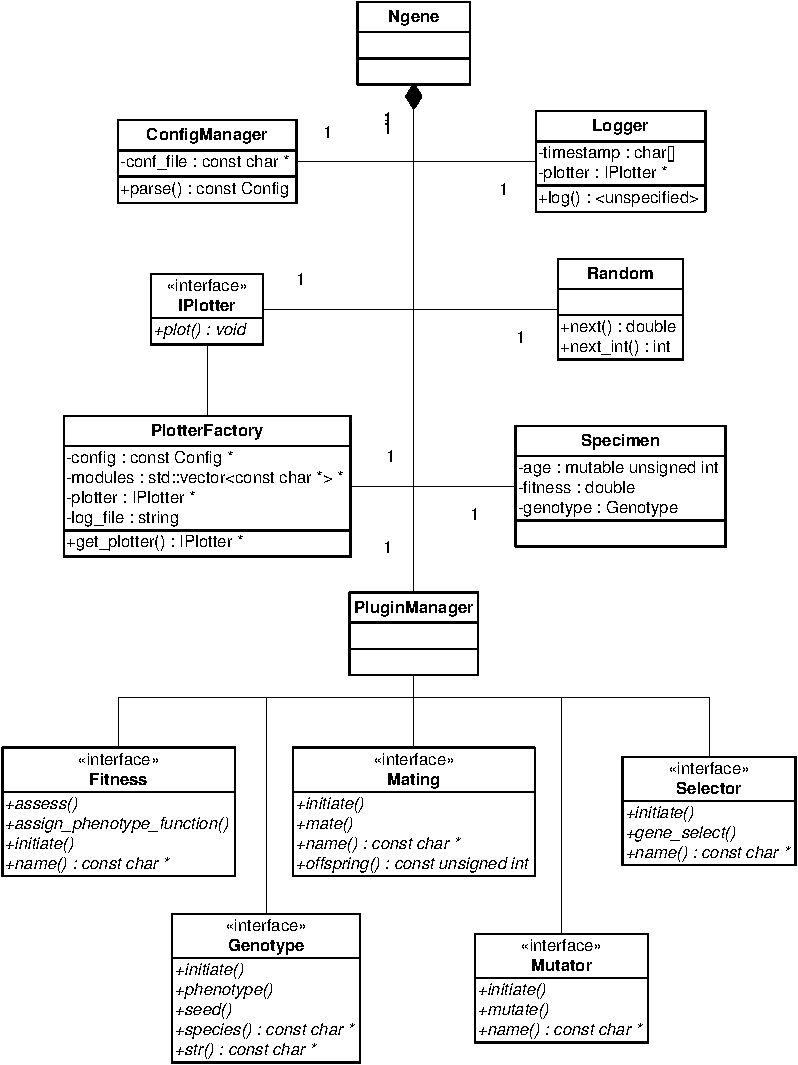
\includegraphics[scale=0.9]{diagram_ngene}
	\caption{Overview of Ngene}
	\label{fig:diagram_ngene}
\end{figure}

Figure~\ref{fig:diagram_ngene} shows a brief overview of how Ngene is put together. At start-up, three of these parts are responsible for what must take place before anything can be run in accordance with the user's parameters. \texttt{ConfigManager} takes care of reading the configuration file and creating a settings object that every other parts have access to. Once the configuration file has been parsed, \texttt{PluginManager} will use this object to find out which modules it's going load. If the user specified tournament selector, it will load the tournament module and make it ready for the genetic engine. When every module is loaded, \texttt{Logger} will use the same settings object to find out how it should log the current run, whether it should plot a fitness/generation graph or just print out the progress on the screen. By now, the genetic algorithm will start. It is a very simple algorithm:

\begin{enumerate}
	\itemsep=0pt
	\item An initial population is randomly generated.
	\item \texttt{Specimen}s are randomly selected for crossover.
	\item Mutate an offspring at random.
	\item Repeat step 2 until the offspring population is of satisfactory size.
	\item Replace adult population with offspring population.
	\item Repeat process from step 2 until the maximum number of generations is reached, or a perfect \texttt{Specimen} is found.
	\item Write log/graph and final \texttt{Specimen} to disk.
\end{enumerate}

The final step is the responsibility of \texttt{Logger}. \texttt{Logger} has no knowledge of what format the \texttt{Specimen} should be written as. Be it a text file, an image or a proprietary format, it will simply request the \texttt{Genotype} module to give it some data to write to disk. The output format is actually coded in each \texttt{Genotype} module because it rarely changes for a single experiment and/or model. Otherwise, a new module must be written anyway.

\texttt{PluginManager}, along with the responsibilities of loading and releasing modules, will also act as a layer between the modules and the genetic engine itself. The engine will never have to bother with the specifics of each module. It should be able to just tell what a module ought to do. Of course, this requires that the modules implement a predefined interface in order to be compatible with this layer. These are described in more detail in the appendix.

\subsection{Ngene Development Framework}
\begin{figure}[!ht]
	\centering
	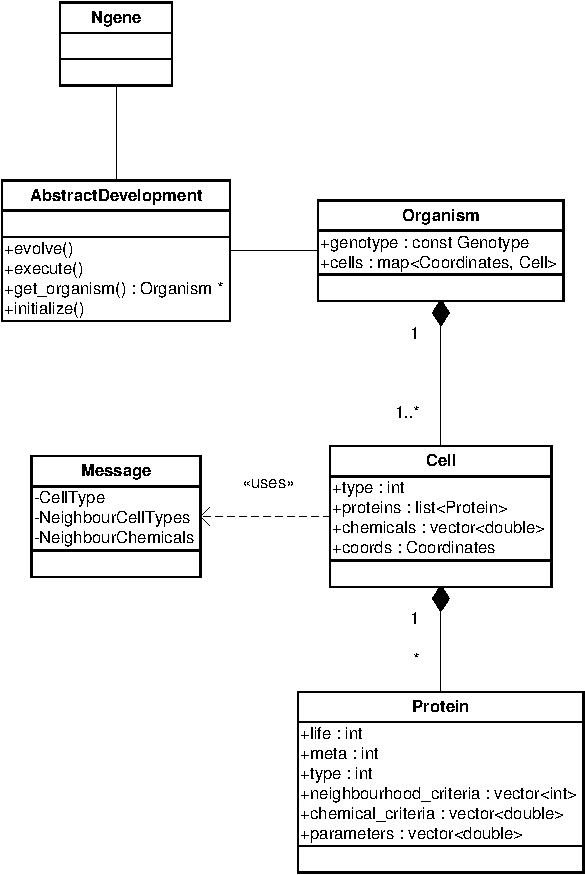
\includegraphics{diagram_ndevframe}
	\caption{Overview of Ngene Development Framework}
	\label{fig:diagram_ndevframe}
\end{figure}

The downside of having such a flexible design, is that users are given too much freedom to implement their own modules. In fact, the engine itself is just a generic genetic algorithm that can be used for any purpose, not just computational development. This will be taken care of by the framework proposed in this thesis.

As mentioned in chapter \ref{sec:framework_requirements}, the framework will provide a code base that will satisfy each and every requirement listed: A development algorithm, message exchange algorithm, and implementations of common concepts such as cells and proteins. The genetic algorithm is already provided for by Ngene. The idea of having such a platform, is to eliminate differing factors that does not have anything to do with the models themselves, and yet does effect the outcome. These are the factors that we need to remove in order to make reliable studies of computational development.

Figure~\ref{fig:diagram_ndevframe} shows how the common concepts are defined. We see that a cell is defined to have a type, some proteins, chemicals and a message storage. These properties may be fixed but users can choose to not use them. ADCGP, for instance, does not make use of proteins. \texttt{AbstractDevelopment} is the class that implements development algorithm. In accordance with the requirements listed in chapter~\ref{sec:framework_requirements}, it implements functions that will allow access to the organism while protecting it: \texttt{divide\_cell()}, \texttt{exists()}, \texttt{queued()}. Respectively, they add a new cell, checks if a cell exists in given location and checks if there will be a new cell in given location. These functions are already implemented and ready to use except for two. Only \texttt{initialize()} and \texttt{execute()} are not. These are the functions that the users will implement their model with. This will be described in more detail in the following subsection.

An intercellular communication algorithm is also included. This works by providing a number of information that can be exchanged. In figure~\ref{fig:diagram_ndevframe_msg}, we see that a message can consist of cell type and chemicals. Some models, say model A may only use the chemicals part of the message while discarding everything else. For model B or C, this might not be the case. As we saw earlier with ArtDev3D and ADCGP, the communication between the two differs a lot. It is important that the message system can provide what is needed for any system and still be able to clearly distinguish the differences so that we can easily take this into consideration when comparing the two models. Use of this code base is enforced in order to ensure that all comparison made between different development models are based on a common ground.

\begin{figure}[!ht]
	\centering
	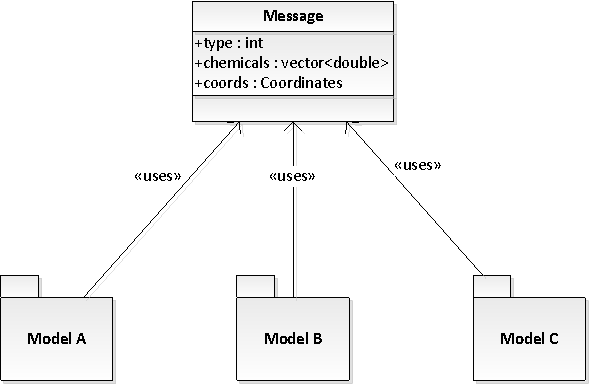
\includegraphics{diagram_ndevframe_msg}
	\caption{A common message implementation should let users easier distinguish the differences in intercellular communication between different models.}
	\label{fig:diagram_ndevframe_msg}
\end{figure}

Figure~\ref{fig:diagram_ndevframe_common-base} demonstrates this requirement. We can see right away that all three models differ because model A and B use chemicals, while C uses proteins. We also see that model B and C require a control program in addition to their cell programs. When models are implemented using the framework, we will be able to clearly see which parts a model uses and why it is unique compared to another model. Since a common code base is used, you can, for example, no longer say that these models produced different results because they ran through different development algorithms. This was the whole point with a common code base from the beginning, it forces users to use it, thus removing this factor.

\begin{figure}[!ht]
	\centering
	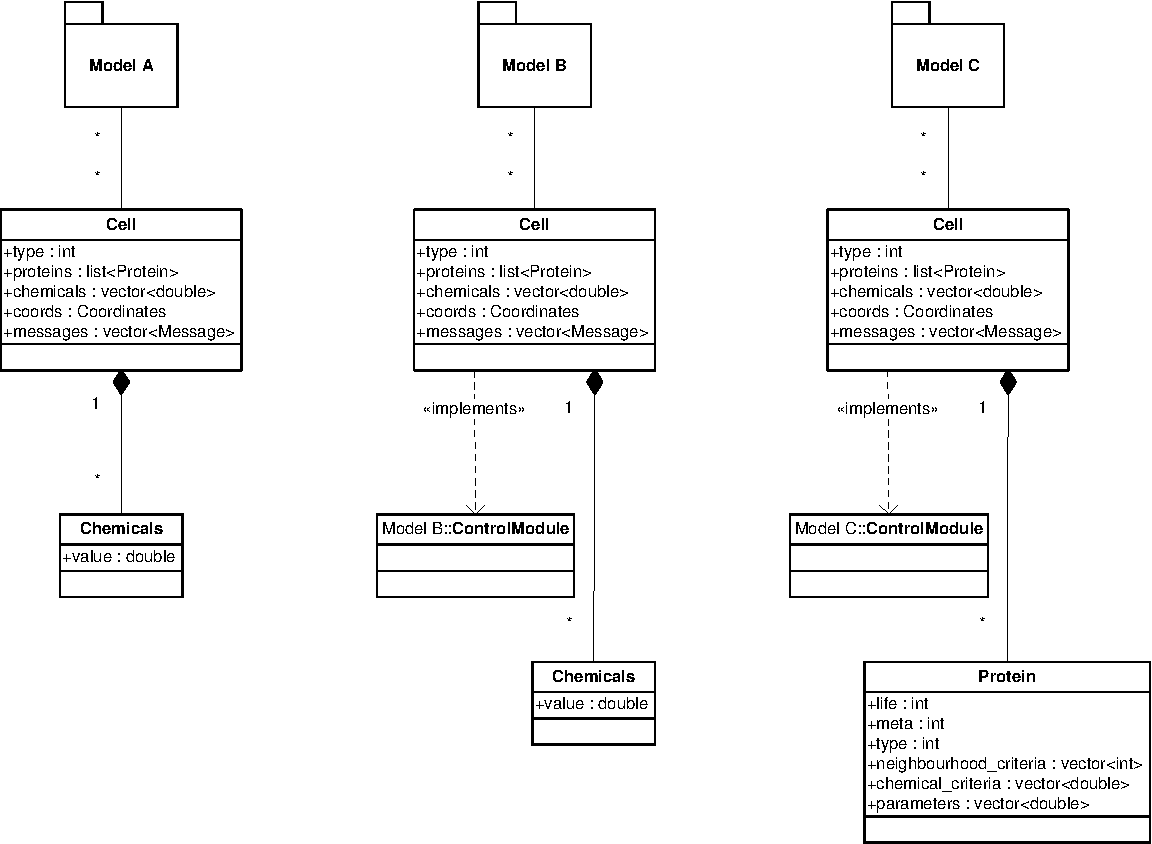
\includegraphics[scale=0.9]{diagram_ndevframe_common-base}
	\caption{Albeit different, all three models still use the same implementation of a cell, chemicals and proteins, and receive the same messages.}
	\label{fig:diagram_ndevframe_common-base}
\end{figure}

Since the framework is going to be used by many users, speed is also a concern when designing it. It is important that the framework is not only flexible and easy to use, but also perform relatively well compared to other implementations. The bottle-neck in these types of systems are usually the representation of the organism. Since lots of CPU time is spent accessing and modifying this object, effort has been spent to figure out how to best represent these organisms. In the current implementation, a C++ Standard Library (STL) \texttt{<map>} is used to store the cells using their coordinates as the key value. It is believed that it keeps the best balance between insertion and lookup time. Alternatives were considered and compared against each other before this decision became final.

\begin{center}
	\begin{tabular}{ r | c | c | c }
		~ & STL \texttt{<map>} & STL \texttt{<vector>} & STL \texttt{<ext/hash\_map>} \\
		\hline
		element access & $O(log~n)$ & $O(1)$ & $O(1)$ \\
		\hline
		insertion & $O(log~n)$ & $O(1)$ & $O(1)$ \\
		\hline
		search & $O(log~n)$ & $O(n)$ & $O(1)$ \\
	\end{tabular}
	\label{tbl:speed}
\end{center}

At first glance, it may seem like the hash map is the best choice to implement the organism with. However, there are some drawbacks that must be taken into consideration. A hash map creates a unique key based on a number of properties found in the value to be stored. The key is used to retrieve the value at some later point. Since the key is meant to be unique for every stored element, the lookup time will be constant ($O(1)$) for any element, regardless of where it is actually stored. This key is creating by a hashing algorithm. The hashing algorithm is essential in both that it determines how uniform the distribution will be over an array, and how well the hash table will perform overall. A too simple hashing algorithm will often experience collisions, i.e.\ a lot of values will be using the same key. When this occurs, there are several ways to handle it. Such a solution is called a collision resolution. One such resolution is to keep values with the same key in a list. This means that when a user wants to retrieve a value, the hash table will have to look through every value in that list. In the worst case scenario, all values will have the same key, suddenly making lookup time linear ($O(n)$) as opposed to theoretical constant time. On the other hand, an overly complex hashing algorithm will also deteriorate performance because more CPU cycles is spent calculating a good hash value. However, regardless of how good the hashing algorithm is, collisions will always occur. The \emph{birthday paradox} predicts that it doesn't take many elements before the chance of a collision exceeds 95\%, even for very big arrays. It is clear that the hash table cannot guarantee its performance advantage over the other containers. Besides, for the experiments conducted in this thesis, the number of cells rarely exceeded 1000. If we use a \texttt{<map>}, which is the case here, it will take at most ten comparisons to find an element by its key value. A good hashing algorithm will use approximately the same number of operations to calculate a key value, perform lookup, and resolve any collisions.

The problem with \texttt{<vector>} is that it is one-dimensional. A drawback is that it will take $O(n)$ time to look for neighbours. This can be worked around by maintaining an up to date neighbours list for every cell. This will make lookup $O(1)$ but increase insertion time to $O(n)$. \texttt{<map>} offers easier facilities to perform such tasks more efficiently. Later, in chapter \ref{sec:improvements}, we will discuss a custom implementation that will theoretically perform better than mentioned containers.

\subsubsection{Using the Framework}
\begin{figure}[!ht]
	\centering
	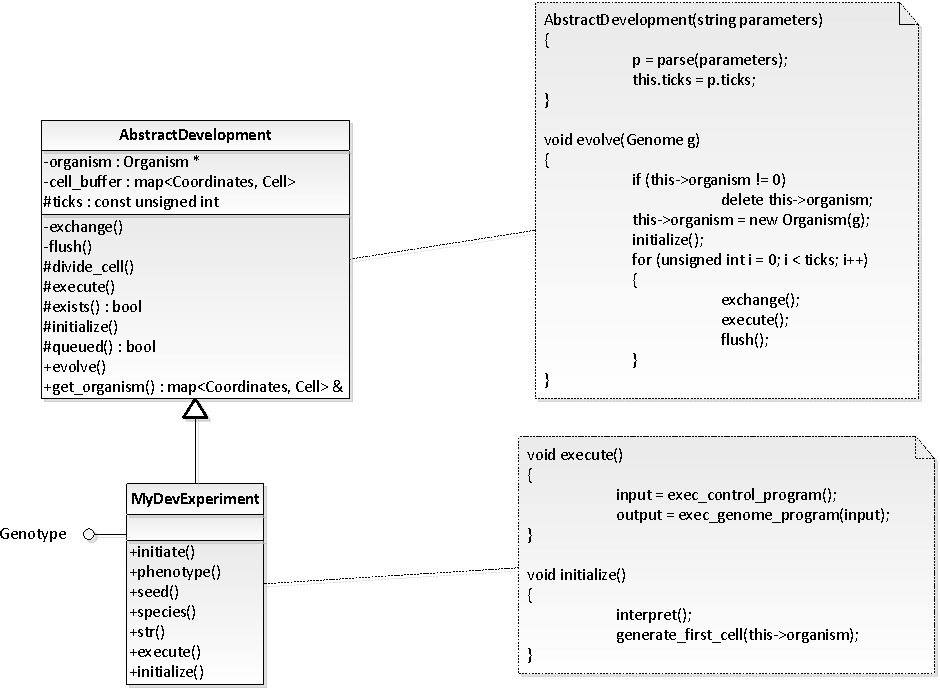
\includegraphics{diagram_ndevframe_ex}
	\caption{An example of how one can implement \texttt{MyDevExperiment}.}
	\label{fig:diagram_ndevframe_ex}
\end{figure}

The framework was designed to ease the implementation effort as much as possible. To start implementing a model, there are some things that need to be considered. First of all, these are the elements that no longer need to be implemented.

\begin{itemize}
	\itemsep=0pt
	\item An evolutionary algorithm (provided by Ngene)
	\item A development algorithm (provided by the framework)
	\item Messaging (provided by the framework)
	\item Cells, chemicals, organisms, proteins, and other concepts (provided by the framework)
\end{itemize}

\noindent The whole code base already provides the basic implementation for any model. The user only needs to focus the following things:

\begin{itemize}
	\itemsep=0pt
	\item\textbf{What does my organism need before development can start?} This can be everything from translating the genotype into a more functional representation (in ADCGP, for example, to make the circuit), creating the first cell(s), to synthesizing proteins (like in ArtDev3D), or setting the chemical level (like in ADCGP). This is what we call the initialization step, and will be implemented in \texttt{initialize()}. This function will be called everytime a new organism is being developed by the framework. The user will never have to concern themselves with how or when to call this function.
	\item\textbf{What does my cell do in a single development step?} This is a focus on a single cell and what it does in a single development step only. For example, with ADCGP, cells create an input string from external signals (received through messages) and feeds the program with the input to get an output that will determine the cells' actions. This is what will go into \texttt{execute()}. Again, as with the other function, this will be called by the framework.
\end{itemize}

\noindent As can be clearly seen, the focus has now shifted on to the models themselves.

Currrently, in order to prevent accidental tampering, there is no way to directly access the organism. A convenience few functions were therefore implemented to remedy this.

\begin{itemize}
	\itemsep=0pt
	\item\texttt{divide\_cell()} lets you tell the organism to add a cell at a given location. These types of calls will be queued up and new cells will not be added before all cells have been executed.
	\item\texttt{exists()} checks if there is a cell at given location in the organism
	\item\texttt{queued()} checks if any other cell has queued a cell to be added at given location, i.e.\ if it has called \texttt{divide\_cell()}.
\end{itemize}

For external signals, the \texttt{messages} array will store information from nearby cells. Note that these are always updated before a development step, and is therefore always up to date.

For the purpose of this thesis, two models were implemented within this framework not only to test the flexibility and performance of this framework but also to see what is missing and what areas need improvement. It is therefore important that these models represent the widest spectrum of computational development.


\subsubsection{ArtDev3D}
\label{sec:Implementation:ArtDev3D}
Porting Johan H{\o}ye's master's thesis\cite{hoye2006} to Ngene's framework has been a matter of finding out what occurs in a cell during a development step, and whether or not there are external processes that needs to be accounted for. As described in chapter~\ref{sec:Models:ArtDev3D}, the genotype of the model does not do all the work in a cell. The cell has its own control program as well. The program can be summarized as the following steps:

\begin{enumerate}
	\itemsep=0pt
	\item Clear all queued actions.
	\item For every active protein, queue their action requests.
	\item Accumulate actions (add them together to execute in one go).
	\item Execute action \#1: Transcribe proteins.
	\item Execute action \#2: Regulate chemical levels.
	\item Execute action \#3: Perform cell division.
	\item Execute action \#4: Change cell type.
	\item Remove dead proteins.
\end{enumerate}

The implementation of the model might seem overwhelming at first impression. There is a heavy use of biological concepts in the code and the simplest operation may span across many classes, and files, as a result. This alone makes it hard to follow the code flow, but the little system documentation that does exist, fortunately, does provide some help although it consists mainly of commentaries in the source files themselves. While his efforts in making it understandable are visible, it might be beneficial to flatten the structure a bit and get rid of some of the redundant structures that are inspired by nature. There is another reason for why this was altered as well.

In theory, such an implementation can have a negative impact on performance. When a simple operation performed must call a function to call another function to call yet another function and so on, can put the calling stack under strain. This may occur because this does not happen only once, but several times every development step in a single cell. And as we know, there are plenty of cells in an organism. Since the model is not concerned with remodeling biology, flattening the structure as mentioned, will reduce the number of calls and potentially improve performance.

\begin{figure}[!ht]
	\centering
	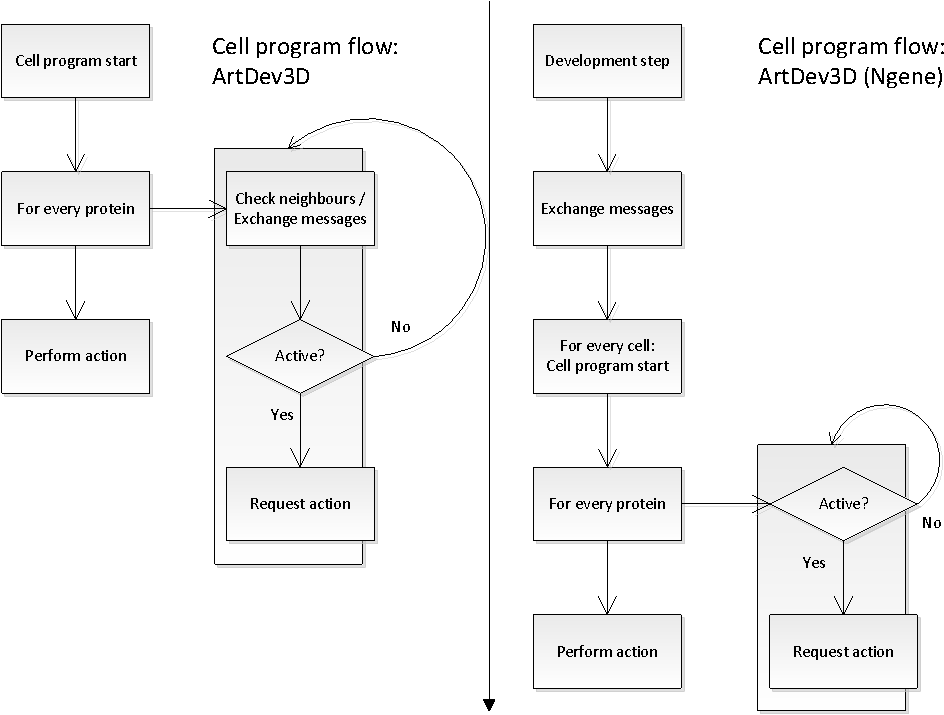
\includegraphics[scale=0.9]{artdev3d_flow}
	\caption{On the left, original ArtDev3D flow. The changed flow on the right.}
	\label{fig:artdev3d_flow}
\end{figure}

There was also an issue that was identified and patched in the port. This was mentioned briefly in \ref{sec:Models:ArtDev3D}. In most models, cells are developed simultaneously. In order to achieve this, information must be exchanged between all cells before a cell can execute its functions. This is to ensure that the control program and DNA will execute based on the current state of the organism without interfering for other cells. In ArtDev3D, this is not properly implemented. The left logical flow in figure~\ref{fig:artdev3d_flow} shows the original ArtDev3D implementation. Upon execution, the cell will start collecting requests from its proteins. The proteins can request an action when they are activated, i.e.\ when the state of the cell and its neighbours are above a threshold. The requests are queued up and then executed. The problem with this, is that it all happens in a single step. Thus, cells that already have had their turn before the current cell, will have an altered state. Actions are therefore based on a mix of ``newer'' information from these cells, and ``old'' information from the rest. When porting this code to the new framework, the cell will no longer have direct access to other cells. Instead, it will receive messages from (or a snapshot of) nearby cells before the development step takes place in any cell. The right logical flow in figure~\ref{fig:artdev3d_flow} is the altered flow of ArtDev3D. Messages are exchanged before any cells are given control. Any action requests are then based on information that does not change as previously. This change may alter the outcome of the model but was addressed because the development algorithm of the framework is already implemented. The model is merely a user of it now.


\subsubsection{Artificial Development (ADCGP)}
\label{sec:cartesian}
This model was implemented from scratch with help from Dr. Julian F. Miller. The model is rather simple because the whole cell program is in the genotype. The implementation should only need to translate the genotype into a working digital circuit and be able to use it.

As we saw in figure~\ref{fig:cartesian_genotype}, the genotype is an array of integers. The number of integers depend on the number of layers and how many nodes each layer consists of. The number of layers and nodes per layer is static. This will keep it simple, and also make the crossover less complicated. As far as I know, this should be in line with Dr. Miller's implementation as well. Each node consists of four integers - three that will serve as connection points to other nodes while the last one will point to a specific function. The function will get its input from the connected nodes' output. The functions implemented here are basic Boolean operations, in addition to the four elementary mathematical operations.

\begin{itemize}
	\itemsep=0pt
	\item \texttt{AND}, \texttt{MUX}, \texttt{NAND}, \texttt{NOR}, \texttt{OR}, \texttt{XNOR}, \texttt{XOR}
	\item addition, division, multiplication, subtraction
\end{itemize}

\noindent Upon initialization, the engine will receive the genotype and will start translating it into a digital circuit. The cell program is then executed:

\begin{itemize}
	\itemsep=0pt
	\item An input bit-string is generated from the chemical levels and types of the current cell together with its neighbours.
	\item The bit-string is sent to the cell program.
	\item The output bit-string is parsed. Some bits will give the cell a new type, the rest will tell the cell to divide in particular directions and how much chemicals these will receive.
	\item The number of chemicals in the cell is adjusted using this formula

	$(c_{ij})_{new} = \frac{1}{2}(c_{ij})_{old} + \frac{1}{16}\sum_{k, l \in N} (c_{kl})_{old}$,

	where $(c_{ij})_{old}$ is the current chemical level, $(c_{ij})_{new}$ is the new chemical level and $\sum_{k, l \in N} (c_{kl})_{old}$ is the sum of the chemical levels in nearby cells (defined as the eight immediate neighbours in 2D grid space).
\end{itemize}

The input bit-string consists of 90 bits. The first 72 bits are the chemical levels in the cell and its eight immediate neighbours (8 bits each). The last 18 bits are the types of the cell and its eight immediate neighbours (2 bits each).

The output bit-string consists of 74 bits. 2 bits denotes the type that the cell changes into. The following 8 bits tells which directions the cell will duplicate itself to (1 bit for each direction). How much chemicals these cells will have are determined by the last 64 bits (8 bits for each direction).

Dr. Miller has also provided with important information regarding his implementation of the model. His implementation actually contains a bug that causes the program to only read the most significant bit from the chemical bits in the neighbours. The other bits are set to zero. When he later identified and patched this bug, he found that the bug was actually beneficial to the model. This bug was also re-implemented in order to make it closer to the original implementation.
